\documentclass[
    ngerman,
    toc=listof,
    toc=bibliography,
    footnotes=multiple,
    parskip=half,
    numbers=noendperiod,
    11pt
]{scrartcl}
\usepackage[utf8]{inputenc}

% !TEX root = ../Projektdokumentation.tex
\newcommand{\titel}{Haupttitel}
\newcommand{\untertitel}{Dies ist der Untertitel}
\newcommand{\kompletterTitel}{\titel{} - \untertitel}
\newcommand{\zeitraum}{1. Januar 2021 - 31. Dezember 2021}

\newcommand{\autorName}{Hendrik Lind}
\newcommand{\autorAnschrift}{Straße 123}
\newcommand{\autorOrt}{12345 Beispielort}
\newcommand{\unterschrift}{images/img_signatureBlue.png}

\newcommand{\logoOben}{images/img_ihk.jpeg}
\newcommand{\logoUnten}{images/img_vbmh.png}
\newcommand{\betriebName}{Testbetrieb}
\newcommand{\betriebAnschrift}{Betriebstraße 110}
\newcommand{\betriebOrt}{12345 Beispielort}

\newcommand{\rahmen}{B. Sc. der Beispielosophie}
\newcommand{\betreff}{Hausarbeit im Modul Beispielkunde}
\newcommand{\pruefungstermin}{Sommersemester 2045}
\newcommand{\abgabeOrt}{Beispielort}
\newcommand{\abgabeTermin}{\today}
% !TEX root = ../Projektdokumentation.tex
\usepackage{setspace} % Spacing einstellen
\usepackage[table,xcdraw]{xcolor} % Tabellen erstellen
\usepackage{etoolbox} % Platz vor Chaptern entfernen

% Anpassung an Landessprache ---------------------------------------------------
\usepackage{babel}

% Umlaute ----------------------------------------------------------------------
%   Umlaute/Sonderzeichen wie äüöß direkt im Quelltext verwenden (CodePage).
%   Erlaubt automatische Trennung von Worten mit Umlauten.
% ------------------------------------------------------------------------------
\usepackage[T1]{fontenc}
\usepackage{textcomp} % Euro-Zeichen etc.

% Schrift ----------------------------------------------------------------------
\usepackage{lmodern} % bessere Fonts
\usepackage{relsize} % Schriftgröße relativ festlegen

% Tabellen ---------------------------------------------------------------------
\PassOptionsToPackage{table}{xcolor}
\usepackage{tabularx}
% für lange Tabellen
\usepackage{longtable}
\usepackage{array}
\usepackage{ragged2e}
\usepackage{lscape}
\newcolumntype{w}[1]{>{\raggedleft\hspace{0pt}}p{#1}} % Spaltendefinition rechtsbündig mit definierter Breite

% Grafiken ---------------------------------------------------------------------
\usepackage[dvips,final]{graphicx} % Einbinden von JPG-Grafiken ermöglichen
\usepackage{graphics} % keepaspectratio
\usepackage{floatflt} % zum Umfließen von Bildern
\graphicspath{{images/}} % hier liegen die Bilder des Dokuments

% Sonstiges --------------------------------------------------------------------
\usepackage[titles]{tocloft} % Inhaltsverzeichnis DIN 5008 gerecht einrücken
\usepackage{amsmath,amsfonts} % Befehle aus AMSTeX für mathematische Symbole
\usepackage{enumitem} % anpassbare Enumerates/Itemizes
\usepackage{xspace} % sorgt dafür, dass Leerzeichen hinter parameterlosen Makros nicht als Makroendezeichen interpretiert werden
\usepackage{booktabs, rotating} % Um bestimmte Seiten anders auszurichten

\usepackage{makeidx} % für Index-Ausgabe mit \printindex
\usepackage[printonlyused]{acronym} % es werden nur benutzte Definitionen aufgelistet

% Einfache Definition der Zeilenabstände und Seitenränder etc.
\usepackage{setspace}
\usepackage{geometry}

% Symbolverzeichnis
\usepackage[intoc]{nomencl}
\let\abbrev\nomenclature
\renewcommand{\nomname}{Abkürzungsverzeichnis}
\setlength{\nomlabelwidth}{.25\hsize}
\renewcommand{\nomlabel}[1]{#1 \dotfill}
\setlength{\nomitemsep}{-\parsep}

\usepackage{varioref} % Elegantere Verweise. „auf der nächsten Seite“
\usepackage{url} % URL verlinken, lange URLs umbrechen etc.

\usepackage{chngcntr} % fortlaufendes Durchnummerieren der Fußnoten
% \usepackage[perpage]{footmisc} % Alternative: Nummerierung der Fußnoten auf jeder Seite neu

\usepackage{ifthen} % bei der Definition eigener Befehle benötigt
\usepackage{todonotes} % definiert u.a. die Befehle \todo und \listoftodos
\usepackage[square]{natbib} % wichtig für korrekte Zitierweise

% PDF-Optionen -----------------------------------------------------------------
\usepackage{pdfpages}
\pdfminorversion=5 % erlaubt das Einfügen von pdf-Dateien bis Version 1.7, ohne eine Fehlermeldung zu werfen (keine Garantie für fehlerfreies Einbetten!)
\usepackage[
    bookmarks,
    bookmarksnumbered,
    bookmarksopen=true,
    bookmarksopenlevel=1,
    colorlinks=true,
% diese Farbdefinitionen zeichnen Links im PDF farblich aus
    anchorcolor=VBMHBlau,% Ankertext
    citecolor=VBMHBlau, % Verweise auf Literaturverzeichniseinträge im Text
    filecolor=VBMHBlau, % Verknüpfungen, die lokale Dateien öffnen
    menucolor=VBMHBlau, % Acrobat-Menüpunkte
    urlcolor=VBMHBlau,
% diese Farbdefinitionen sollten für den Druck verwendet werden (alles schwarz)
    %linkcolor=black, % einfache interne Verknüpfungen
    %anchorcolor=black, % Ankertext
    %citecolor=black, % Verweise auf Literaturverzeichniseinträge im Text
    %filecolor=black, % Verknüpfungen, die lokale Dateien öffnen
    %menucolor=black, % Acrobat-Menüpunkte
    %urlcolor=black,
%
    %backref, % Quellen werden zurück auf ihre Zitate verlinkt
    pdftex,
    plainpages=false, % zur korrekten Erstellung der Bookmarks
    pdfpagelabels=true, % zur korrekten Erstellung der Bookmarks
    hypertexnames=false, % zur korrekten Erstellung der Bookmarks
    linkcolor=black,
    linktoc=all,
]{hyperref}
% Befehle, die Umlaute ausgeben, führen zu Fehlern, wenn sie hyperref als Optionen übergeben werden
\hypersetup{
    pdftitle={\titel -- \untertitel},
    pdfauthor={\autorName},
    pdfcreator={\autorName},
    pdfsubject={\titel -- \untertitel},
    pdfkeywords={\titel -- \untertitel},
}


% zum Einbinden von Programmcode -----------------------------------------------
\usepackage{listings}
\usepackage{xcolor}
\definecolor{hellgelb}{rgb}{1,1,0.9}
\definecolor{colKeys}{rgb}{0,0,1}
\definecolor{colIdentifier}{rgb}{0,0,0}
\definecolor{colComments}{rgb}{0,0.5,0}
\definecolor{colString}{rgb}{1,0,0}
\lstset{
    float=hbp,
	basicstyle=\footnotesize,
    identifierstyle=\color{colIdentifier},
    keywordstyle=\color{colKeys},
    stringstyle=\color{colString},
    commentstyle=\color{colComments},
    backgroundcolor=\color{hellgelb},
    columns=flexible,
    tabsize=2,
    frame=single,
    extendedchars=true,
    showspaces=false,
    showstringspaces=false,
    numbers=left,
    numberstyle=\tiny,
    breaklines=true,
    breakautoindent=true,
	captionpos=b,
}
\lstdefinelanguage{cs}{
	sensitive=false,
	morecomment=[l]{//},
	morecomment=[s]{/*}{*/},
	morestring=[b]",
	morekeywords={
		abstract,event,new,struct,as,explicit,null,switch
		base,extern,object,this,bool,false,operator,throw,
		break,finally,out,true,byte,fixed,override,try,
		case,float,params,typeof,catch,for,private,uint,
		char,foreach,protected,ulong,checked,goto,public,unchecked,
		class,if,readonly,unsafe,const,implicit,ref,ushort,
		continue,in,return,using,decimal,int,sbyte,virtual,
		default,interface,sealed,volatile,delegate,internal,short,void,
		do,is,sizeof,while,double,lock,stackalloc,
		else,long,static,enum,namespace,string},
}
\lstdefinelanguage{natural}{
	sensitive=false,
	morecomment=[l]{/*},
	morestring=[b]",
	morestring=[b]',
	alsodigit={-,*},
	morekeywords={
		DEFINE,DATA,LOCAL,END-DEFINE,WRITE,CALLNAT,PARAMETER,USING,
		IF,NOT,END-IF,ON,*ERROR-NR,ERROR,END-ERROR,ESCAPE,ROUTINE,
		PERFORM,SUBROUTINE,END-SUBROUTINE,CONST,END-FOR,END,FOR,RESIZE,
		ARRAY,TO,BY,VALUE,RESET,COMPRESS,INTO,EQ},
}
\lstdefinelanguage{php}{
	sensitive=false,
	morecomment=[l]{/*},
	morestring=[b]",
	morestring=[b]',
	alsodigit={-,*},
	morekeywords={
		abstract,and,array,as,break,case,catch,cfunction,class,clone,const,
		continue,declare,default,do,else,elseif,enddeclare,endfor,endforeach,
		endif,endswitch,endwhile,extends,final,for,foreach,function,global,
		goto,if,implements,interface,instanceof,namespace,new,old_function,or,
		private,protected,public,static,switch,throw,try,use,var,while,xor
		die,echo,empty,exit,eval,include,include_once,isset,list,require,
		require_once,return,print,unset},
}

\usepackage{lipsum}

% !TEX root = ../Projektdokumentation.tex

% Befehle für häufig anfallende Aufgaben
\newcommand{\Abbildung}[1]{\autoref{fig:#1}}
\newcommand{\Anhang}[1]{\appendixname{}~\ref{#1}: \nameref{#1} \vpageref{#1}}
\newcommand{\includegraphicsKeepAspectRatio}[2]{\includegraphics[width=#2\textwidth,height=#2\textheight,keepaspectratio]{#1}}
\newcommand{\Zitat}[2][\empty]{\ifthenelse{\equal{#1}{\empty}}{\citep{#2}}{\citep[#1]{#2}}}
\newcommand{\Autor}[1]{\textsc{#1}} % zum Ausgeben von Autoren
\newcommand{\itemd}[2]{\item{\textbf{#1}}\\{#2}} % erzeugt ein Listenelement mit fetter Überschrift

% fügt Tabellen aus einer TEX-Datei ein
\newcommand{\tabelle}[3] % Parameter: caption, label, file
{\begin{table}[htbp]
\centering
\singlespacing
\input{tables/tab_#3}
\caption{#1}
\label{#2}
\end{table}}

\newcommand{\tabelleAnhang}[1] % Parameter: file
{\begin{center}
\singlespacing
\input{tables/tab_#1}
\end{center}}

% einfaches Wechseln der Schrift, z.B.: \changefont{cmss}{sbc}{n}
\newcommand{\changefont}[3]{\fontfamily{#1} \fontseries{#2} \fontshape{#3} \selectfont}

% Verwendung analog zu \includegraphics
\newlength{\myx} % Variable zum Speichern der Bildbreite
\newlength{\myy} % Variable zum Speichern der Bildhöhe
\newcommand\includegraphicstotab[2][\relax]{%
% Abspeichern der Bildabmessungen
\settowidth{\myx}{\includegraphics[{#1}]{#2}}%
\settoheight{\myy}{\includegraphics[{#1}]{#2}}%
% das eigentliche Einfügen
\parbox[c][1.1\myy][c]{\myx}{%
\includegraphics[{#1}]{#2}}%
}

\definecolor{VBMHBlau}{rgb}{0, 96, 170}
\definecolor{VBMHOrange}{rgb}{236, 105, 31}

% verschiedene Befehle um Wörter semantisch auszuzeichnen ----------------------
\newcommand{\Index}[2][\empty]{\ifthenelse{\equal{#1}{\empty}}{\index{#2}#2}{\index{#1}#2}}
\newcommand{\Fachbegriff}[2][\empty]{\ifthenelse{\equal{#1}{\empty}}{\textit{\Index{#2}}}{\textit{\Index[#1]{#2}}}}
\newcommand{\NeuerBegriff}[2][\empty]{\ifthenelse{\equal{#1}{\empty}}{\textbf{\Index{#2}}}{\textbf{\Index[#1]{#2}}}}

\newcommand{\Ausgabe}[1]{\texttt{#1}}
\newcommand{\Eingabe}[1]{\texttt{#1}}
\newcommand{\Code}[1]{\texttt{#1}}
\newcommand{\Datei}[1]{\texttt{#1}}

\newcommand{\Assembly}[1]{\textsf{#1}}
\newcommand{\Klasse}[1]{\textsf{#1}}
\newcommand{\Methode}[1]{\textsf{#1}}
\newcommand{\Attribut}[1]{\textsf{#1}}

\newcommand{\Datentyp}[1]{\textsf{#1}}
\newcommand{\XMLElement}[1]{\textsf{#1}}
\newcommand{\Webservice}[1]{\textsf{#1}}

\newcommand{\Refactoring}[1]{\Fachbegriff{#1}}
\newcommand{\CodeSmell}[1]{\Fachbegriff{#1}}
\newcommand{\Metrik}[1]{\Fachbegriff{#1}}
\newcommand{\DesignPattern}[1]{\Fachbegriff{#1}}

\newcommand{\vbmh}{\ac{VBMH}} 
% !TEX root = ../Projektdokumentation.tex

% Vorgaben IHK -----------------------------------------------------------------
% Schriftgröße: 11
% Zeilenabstand: 1,5 zeilig
% Rand: 2,5 cm (links, rechts, oben, unten)
% Ausrichtung: Blocksatz --> Standardmäßig in LaTeX aktiv
% Seitenzahlen: Fußzeile, zentriert, beginnend mit der Dokumentation
% Maximale Tiefe: 1.1.1 / subsubsections

\geometry{a4paper, margin=25mm}

\usepackage[
	automark, % Kapitelangaben in Kopfzeile automatisch erstellen
	headsepline, % Trennlinie unter Kopfzeile
	ilines % Trennlinie linksbündig ausrichten
]{scrlayer-scrpage}

\pagestyle{scrheadings}

% Kopfzeile ---------------------------------------------------------------------
\renewcommand*\sectionmarkformat{} % Keine Nummerierung im Kopf
\renewcommand{\headfont}{\normalfont} % Schriftform der Kopfzeile
\ihead{\large{\titel}\\[1ex] \textit{\headmark}}
\automark{section}
\chead{}
\ohead{\includegraphics[scale=0.2]{\betriebLogo}}
\setlength{\headheight}{15mm} % Höhe der Kopfzeile

% Fußzeile ---------------------------------------------------------------------
\ifoot{\autorName}
\cfoot{\pagemark}
\ofoot{\betriebName}
\setlength{\footheight}{10mm} % Höhe der Fußzeile

% Abstand zwischen Nummerierung und Überschrift definieren
\newcommand{\headingSpace}{1.0 cm}

% Abschnittsüberschriften im selben Stil wie beim Inhaltsverzeichnis einrücken
\renewcommand*{\othersectionlevelsformat}[3]{
  \makebox[\headingSpace][l]{#3\autodot}
}

%\cftsetindents{chapter}{0.0cm}{\headingSpace}
\cftsetindents{section}{0.0cm}{\headingSpace}
\cftsetindents{subsection}{1.0cm}{1.0 cm}
\cftsetindents{subsubsection}{2.0cm}{1.45 cm}
\cftsetindents{figure}{0.0cm}{\headingSpace}
\cftsetindents{table}{0.0cm}{\headingSpace}


% Allgemeines -----------------------------------------------------------------

\setlength{\textheight}{665pt} % Größe des "Textfeldes"

\onehalfspacing % Zeilenabstand 1,5 Zeilen
\frenchspacing % erzeugt ein wenig mehr Platz hinter einem Punkt

\usepackage{blindtext} % Lipsum

\counterwithout{footnote}{section} % Fußnoten fortlaufend durchnummerieren
\setcounter{tocdepth}{3} % im Inhaltsverzeichnis werden die Kapitel bis zum Level der subsubsection übernommen
\setcounter{secnumdepth}{3} % Kapitel bis zum Level der subsubsection werden nummeriert

% Aufzählungen anpassen
\renewcommand{\labelenumi}{\arabic{enumi}.}
\renewcommand{\labelenumii}{\arabic{enumi}.\arabic{enumii}.}
\renewcommand{\labelenumiii}{\arabic{enumi}.\arabic{enumii}.\arabic{enumiii}}

% Tabellenfärbung
\definecolor{heading}{rgb}{0.64,0.78,0.86}
\definecolor{odd}{rgb}{0.9,0.9,0.9}

\usepackage{float}




  
\begin{document}
    % Deckblatt --------------------------------------------------------------
    \phantomsection
    \thispagestyle{plain}
    \pdfbookmark[1]{Deckblatt}{deckblatt}
    % !TEX root = Projektdokumentation.tex
\begin{titlepage}
    
\begin{figure}[t]
    \centering
    \includegraphics[width=5cm,keepaspectratio]{\logoOben}
    \label{fig:ihk1}	
\end{figure}
    
\begin{center}
    {\large \pruefungstermin} \\[2em]
    	
    {\Large \rahmen} \\[1em]
    {\Large \betreff} \\[5em]
    	
    \textbf{\huge \titel} \\[1em]
    \textbf{\Large \untertitel} \\[4em]
    	
    \textbf{Durchführungszeitraum:} \zeitraum\\[2em]
    	
    \textbf{Autor:}\\
    \autorName\\
    \autorAnschrift\\
    \autorOrt\\
\end{center}
    
\begin{figure}[h]
    \centering
    \includegraphics[width=8cm,keepaspectratio]{\logoUnten}
    \label{fig:vbmh1}
\end{figure}
    
\begin{center}
    \textbf{Betrieb/Hochschule:}\\
    \betriebName\\
    \betriebAnschrift\\
    \betriebOrt\\
\end{center}
    
\end{titlepage}
    \cleardoublepage
    
    % Inhaltsverzeichnis -----------------------------------------------------
    \phantomsection
    \newcounter{savepage}
    \pagenumbering{roman}
    \addcontentsline{toc}{section}{Inhaltsverzeichnis}
    \tableofcontents
    \cleardoublepage
    
    % Abbildungsverzeichnis (kein Page-Break) --------------------------------
    \phantomsection
    \listoffigures
    
    % Tabellenverzeichnis ----------------------------------------------------
    \phantomsection
    \listoftables
    \cleardoublepage
    
    % Abkürzungsverzeichnis --------------------------------------------------
    \phantomsection
    \newcommand{\abkvz}{Abkürzungsverzeichnis}
    \renewcommand{\nomname}{\abkvz}
    \section*{\abkvz}
    \markboth{\abkvz}{\abkvz}
    \addcontentsline{toc}{section}{Abkürzungsverzeichnis}
    % !TEX root = Projektdokumentation.tex

% Definieren mit \ac
% Keine automatische Anordnung nach dem Alphabet möglich --> per Excel manuell erledigen

\begin{acronym}\itemsep-15pt
    \acro{BSP}[BSP]{Beispiel}
    \acroplural{BSP}[BSPs]{Beispiele}
\end{acronym}
    \clearpage
    
    %Hyperlink Color
    \definecolor{hyperref}{RGB}{0,68,102}
    \hypersetup{
    linkcolor = hyperref,
    anchorcolor = hyperref,
    citecolor = hyperref,
    filecolor = hyperref,
    urlcolor = hyperref
    }
    
    % Inhalt -----------------------------------------------------------------
    \setcounter{savepage}{\arabic{page}}
    \pagenumbering{arabic}
    % !TEX root = Projektdokumentation.tex
% !TEX root = ../Projektdokumentation.tex
\section{Einleitung}
\label{sec:Einleitung}
\lipsum[1]

    \subsection{Unterleitung}
    \label{sec:Unterleitung}
    \lipsum[3]
    Siehe als \ac{BSP} im Anhang unter \ref{app:Codebeispiel}.
    \lipsum[1]
    \cite{BSPLIT}
% !TEX root = ../Projektdokumentation.tex
\section{Hauptteil}
\label{sec:Hauptteil}
\lipsum[3]

% !TEX root = ../Projektdokumentation.tex
\section{Fazit}
\label{sec:Fazit}
\lipsum[3]
    
    % Literatur ------------------------------------------------------------------
    \clearpage
    \pagenumbering{roman}
    \setcounter{page}{\thesavepage}
    \begin{thebibliography}{9}

% Einleitung
\bibitem{BSPLIT}
Beispiel Web-Zitat, Abgerufen am 24.12.2021 \url{https://www.google.de}

\end{thebibliography}
    \clearpage
    
    % Anhang -----------------------------------------------------------------
    \clearpage
    \appendix
    \setcounter{savepage}{\arabic{page}}
    \pagenumbering{Roman}
    % !TEX root = Projektdokumentation.tex


\section{Anhang}
    \subsection{Detaillierte Zeitplanung}
    \label{app:Zeitplanung}
    \begin{table}[ht]
        \tabelleAnhang{ZeitplanungKomplett}
        \caption{Detaillierte Zeitplanung}
    \end{table}
    
    \subsection{Beispielauflistung}
    \label{app:Beispielauflistung}
    Hardware
    \begin{itemize}
        \item Mobiler Arbeitsplatz (HP EliteBook 840 G5)
        \item 	Zwei Monitore
    \end{itemize}
    
    %/pagebreak
    
    \subsection{Beispielbild}
    \label{app:Excel}

    \begin{figure}[H]
        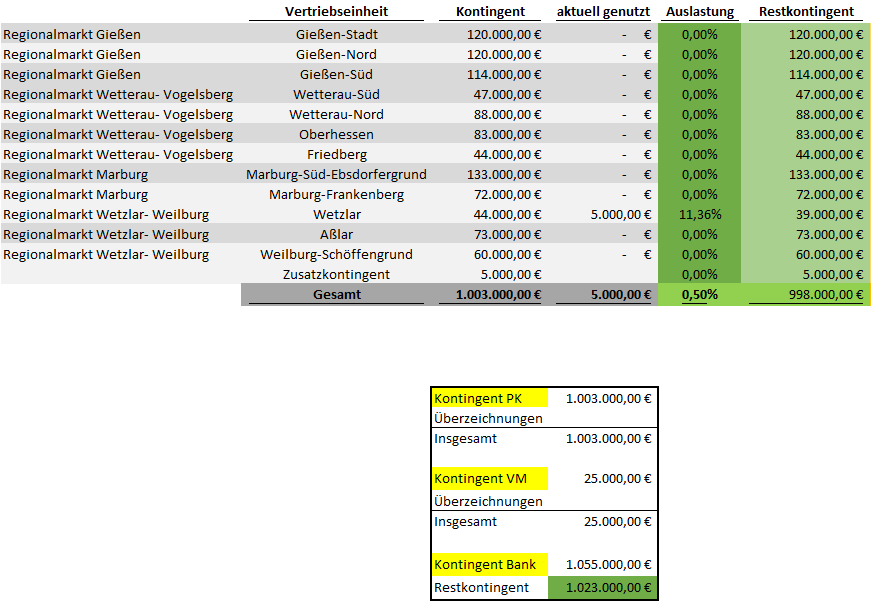
\includegraphics[width=\textwidth,height=\textheight,keepaspectratio]{images/img_exceltable.png}
        \caption{Ausschnitt Excel-Dokument}
    \end{figure}

    \subsection{Beispieltabelle}
    \label{app:Beispieltabelle}
    \begin{table}[ht]
        \tabelleAnhang{Kostenplanung}
        \caption{Kostenplanung}
    \end{table}
    
    \subsection{Berechnung}
    \label{app:Berechnung}
    
    \begin{equation}
    \label{app:BerechnungX}
        \begin{array}{1}
            Jährliche\;Zeitersparnis = 555\;Minuten/Monat\;*\; 6.660\;Minuten/Jahr = 111\;Stunden/Jahr\\
            Jährlicher\:Rückfluss = 111\:Stunden/Jahr * 60\:Euro/Stunde = 6.660 Euro\\
            Amortisationsdauer = 7.040\;Euro Kosten/6.660\;Euro Rückfluss = 1,057\;Jahre
        \end{array}
    \end{equation}

     \subsection{Code-Beispiele}
     \label{app:Codebeispiele}
         

    \subsubsection{Codebeispiel}
    \label{app:Codebeispiel}
    \definecolor{lightgrey}{rgb}{0.9,9, 0.9} % 0.8, 0.8, 1 --> lightpurple
    
        \lstset{
    	numbers=left,
    	stepnumber=1,
    	numbersep=5pt,
    	numberstyle=\small\color{black},
    	basicstyle=\ttfamily,
    	keywordstyle=\color{black},
    	commentstyle=\color{black},
    	stringstyle=\color{black},
    	frame=single,
    	tabsize=3,
    	backgroundcolor=\color{lightgrey}}
    
    \begin{lstlisting}
        var x = 12345
    \end{lstlisting}

    
    % Erklärung --------------------------------------------------------------
    \clearpage
    \phantomsection
    \pagenumbering{roman}
    \setcounter{page}{\thesavepage}
    % !TEX root = Projektdokumentation.tex
\clearpage
\addsec{Eidesstattliche Erklärung}

Ich, \autorName, versichere hiermit, dass ich meine \textbf{\betreff} mit dem
Thema
\begin{quote}
\textit{\kompletterTitel}
\end{quote}
selbständig verfasst und keine anderen als die angegebenen Quellen und Hilfsmittel benutzt habe, wobei ich alle wörtlichen und sinngemäßen Zitate als solche gekennzeichnet habe. Die Arbeit wurde bisher keiner anderen Prüfungsbehörde vorgelegt und auch nicht veröffentlicht.\\[6ex]

\abgabeOrt, den \abgabeTermin

\includegraphics[scale=0.4]{\unterschrift}
\par 	
\vspace{-1.1cm}

\rule[-0.2cm]{5.5cm}{0.5pt}

\textsc{\autorName}

    \cleardoublepage
    
\end{document}
